\documentclass[11pt,letterpaper]{article}
\usepackage[margin=0.72in,headheight=14pt,headsep=13pt,footskip=23pt]{geometry}
\usepackage{fontspec}
\usepackage{amsmath,amssymb,graphicx,booktabs,tabularx,float,xcolor}
\usepackage{caption,fancyhdr,titlesec}
\usepackage[unicode,hidelinks]{hyperref}
\hypersetup{pdftitle={Continuous- and Discrete-Time PINNs in PyTorch},pdfauthor={Shang Gao}}
\definecolor{ink}{HTML}{000000}
\definecolor{muted}{HTML}{000000}
\setlength{\parindent}{0pt}
\setlength{\parskip}{5pt}
\linespread{1.02}
\setlength{\abovedisplayskip}{6pt}
\setlength{\belowdisplayskip}{6pt}
\setlength{\intextsep}{8pt}
\captionsetup{font=small,labelfont=bf,skip=4pt}
\titleformat{\section}{\large\bfseries\color{ink}}{\thesection}{.6em}{}
\titlespacing*{\section}{0pt}{8pt}{4pt}
\pagestyle{fancy}\fancyhf{}
\fancyhead[L]{\small\color{muted}CEE 292 \quad PINNs in PyTorch}
\fancyhead[R]{\small\color{muted}Shang Gao}
\fancyfoot[C]{\small\thepage}
\renewcommand{\headrulewidth}{0.3pt}
\newcommand{\projecturl}{https://github.com/shang698/pinns-pytorch}
\newcommand{\projectlink}{\href{\projecturl}{\expandafter\nolinkurl\expandafter{\projecturl}}}
\begin{document}
\thispagestyle{plain}
{\centering\bfseries\fontsize{16}{19}\selectfont CEE 292 Scientific Machine Learning\par}
\vspace{5pt}
{Course Project Report\hfill\textbf{Shang Gao}\par}
\vspace{4pt}\hrule height .4pt\vspace{9pt}
{\color{ink}\bfseries\fontsize{17}{21}\selectfont Continuous- and Discrete-Time PINNs in PyTorch:\\Reproduction and Double-Precision Refinement\par}
\vspace{6pt}
\textbf{Paper.} \emph{Physics-informed neural networks: A deep learning framework for solving forward and inverse problems involving nonlinear partial differential equations}. Raissi et al. (2019) combine observations with PDE constraints through continuous- and discrete-time neural networks~\cite{raissi}.

\textbf{My contribution.} I implemented the Schr\"odinger and Allen--Cahn forward examples in PyTorch, using the authors' TensorFlow code as a reference, and compared float32 and float64 refinement from the same trained weights.

\section{Methods and experimental setup}
\textbf{Continuous time: Schr\"odinger.} The complex field $h=u+iv$ satisfies
\begin{equation}
 i h_t+\tfrac12 h_{xx}+|h|^2h=0,\qquad x\in[-5,5],\quad t\in[0,\pi/2].
\end{equation}
The initial condition is $h(x,0)=2\,\mathrm{sech}(x)$, with periodic $h$ and $h_x$. A network maps $(x,t)$ to $(u,v)$. PyTorch automatic differentiation evaluates the PDE residual $r=i h_t+\tfrac12h_{xx}+|h|^2h$. Training minimizes the sum of initial-data, periodic-boundary, and residual mean-squared errors. Real and imaginary contributions are both included.

\textbf{Discrete time: Allen--Cahn.} Here the equation is $u_t=F(u)=10^{-4}u_{xx}+5u-5u^3$ on $x\in[-1,1]$, with periodic values and derivatives. Following the published example, I use 200 observations at $t_n=0.1$ to predict $t_{n+1}=0.9$ in one step, $\Delta t=0.8$. A network takes $x$ and returns 100 implicit Runge--Kutta (IRK) stages and the final solution. With the authors' coefficients,
\begin{equation}
\begin{aligned}
 R_i(x)&=U_i(x)-\Delta t\sum_{j=1}^{100}a_{ij}F(U_j(x)),\quad i=1,\ldots,100,\\
 R_{101}(x)&=U_{101}(x)-\Delta t\sum_{j=1}^{100}b_jF(U_j(x)).
\end{aligned}
\end{equation}
All $R_i$ are fitted to the same earlier snapshot. The loss sums squared data errors and periodic value and derivative errors over all outputs, as in the original code.

\begin{table}[H]\centering\small
\caption{Baseline configuration. Both networks use $\tanh$ hidden layers and linear outputs.}
\begin{tabularx}{\linewidth}{@{}lXX@{}}\toprule
 & Schr\"odinger & Allen--Cahn \\\midrule
Network widths & $[2,100,100,100,100,2]$ & $[1,200,200,200,200,101]$ \\
Training data & 50 initial points; 50 boundary times; 20,000 residual points & 200 points at $t=0.1$; periodic constraints at $x=\pm1$ \\
Adam steps & 50,000 & 10,000 \\
L-BFGS-B budget & \multicolumn{2}{l}{Up to 50,000 iterations and 50,000 function evaluations} \\\bottomrule
\end{tabularx}
\end{table}
I used the authors' public \texttt{NLS.mat}, \texttt{AC.mat}, and 100-stage IRK table~\cite{code}. Snapshot observations enter training only at $t=0$ for Schr\"odinger and $t=0.1$ for Allen--Cahn. Both baselines use float32, seed 1234, input scaling to $[-1,1]$, and Adam with learning rate $10^{-3}$, followed by SciPy L-BFGS-B using PyTorch gradients. Its tolerances are $\mathrm{gtol}=10^{-5}$ and $\mathrm{ftol}=2.22\times10^{-16}$; history size and maximum line-search steps are both 50.

\clearpage
\section{Reproduction results}
I evaluate relative $L^2$ error, $\mathcal E=\|\hat y-y\|_2/\|y\|_2$, using the complete reference grid: $256\times201$ space--time points for Schr\"odinger and 512 points at $t=0.9$ for Allen--Cahn. For Schr\"odinger, I report both amplitude and complex-solution errors to measure errors in both magnitude and phase.
\begin{table}[H]\centering\small
\caption{Relative $L^2$ errors (\%). Paper values are from Figures 1 and 2 of~\cite{raissi}.}\label{tab:errors}
\begin{tabularx}{\linewidth}{@{}Xrrrr@{}}\toprule
 & Paper & PyTorch & \multicolumn{2}{c}{Continuation} \\
Quantity & reference & baseline & float32 & float64 \\\midrule
Schr\"odinger amplitude $|h|$ & 0.197 & 0.101 & 0.100 & 0.0954 \\
Schr\"odinger complex field $h$ & -- & 0.143 & 0.143 & 0.132 \\
Allen--Cahn, $t=0.9$ & 0.699 & 0.391 & 0.391 & 0.317 \\\bottomrule
\end{tabularx}
\end{table}
\begin{figure}[H]\centering
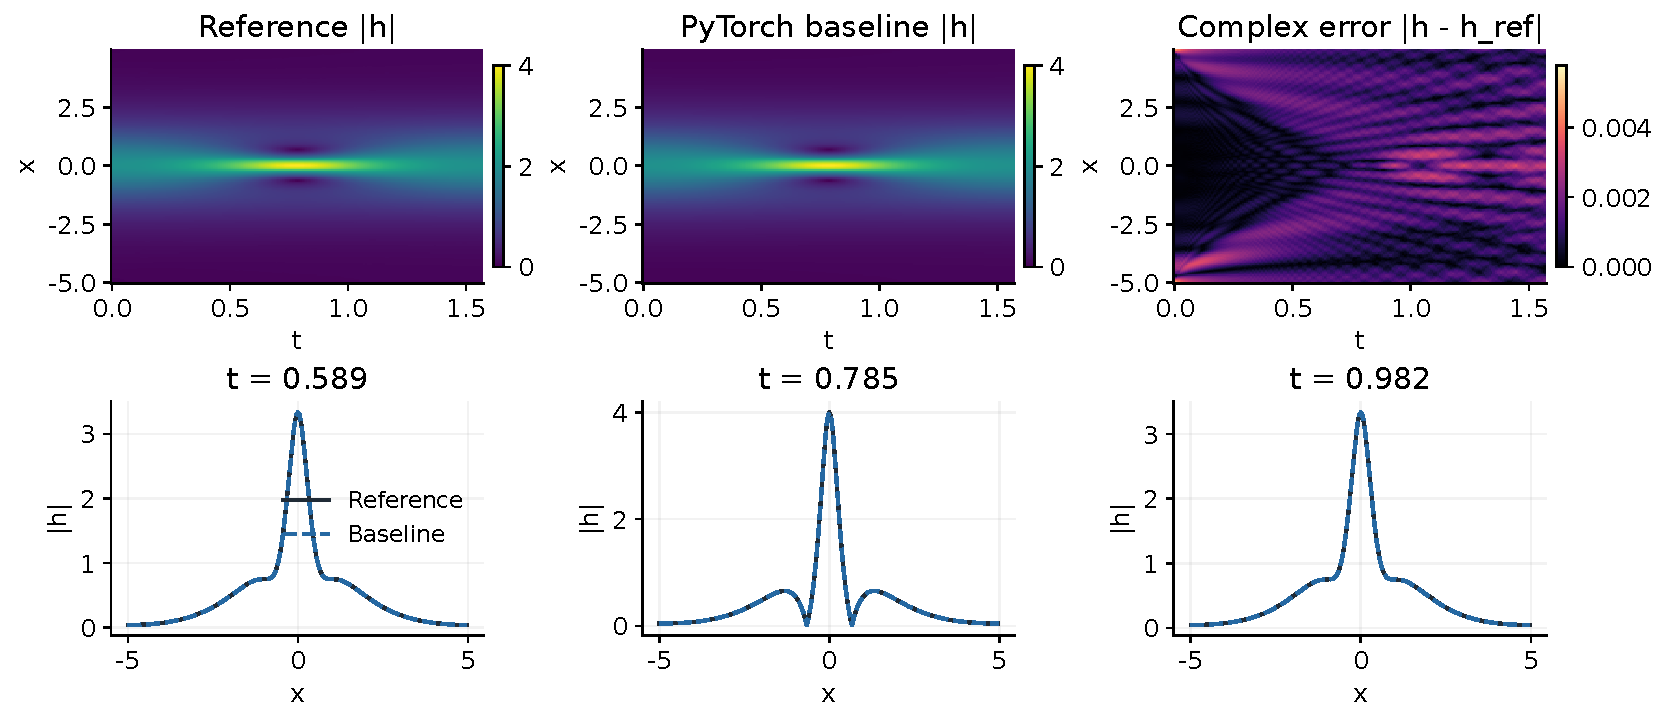
\includegraphics[width=\linewidth]{images/nls_baseline.pdf}
\caption{Schr\"odinger baseline: reference and predicted amplitudes, absolute complex error, and three amplitude slices.}\label{fig:nls}
\end{figure}
\begin{figure}[H]\centering
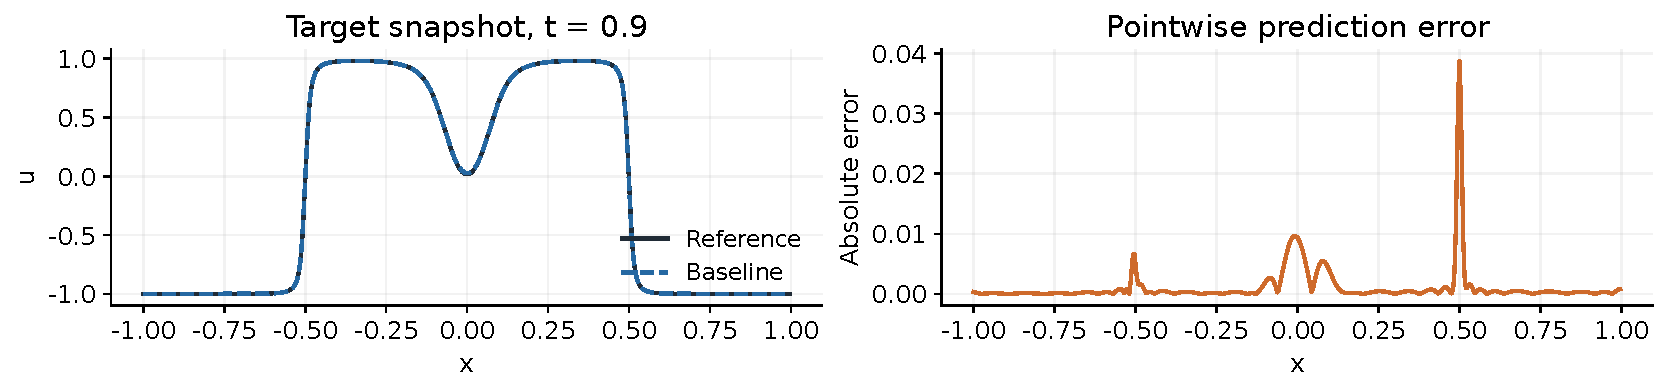
\includegraphics[width=\linewidth]{images/ac_baseline.pdf}
\caption{Allen--Cahn baseline at $t=0.9$: solution profile and pointwise absolute error.}\label{fig:ac}
\end{figure}
Both baselines have lower errors than the paper's reference values. The largest Allen--Cahn error is near $x=0.5$, with smaller errors around the center and the left transition. L-BFGS-B stopped after 8,126 iterations for Schr\"odinger and 14,852 for Allen--Cahn, on the relative objective-decrease criterion rather than the gradient tolerance. Neither used the full 50,000-iteration budget. This early stopping motivated the continuation experiment.
\clearpage
\section{Double-precision refinement}
For each baseline, I restarted L-BFGS-B from the same final weights in float32 and float64, using identical training points and a fresh optimizer history. No further Adam steps were taken. Both arms used $\mathrm{gtol}=10^{-8}$, at most 5,000 iterations and 7,500 function evaluations; other optimizer settings were unchanged. Allen--Cahn's IRK coefficients used the selected precision as well.

\begin{figure}[H]\centering
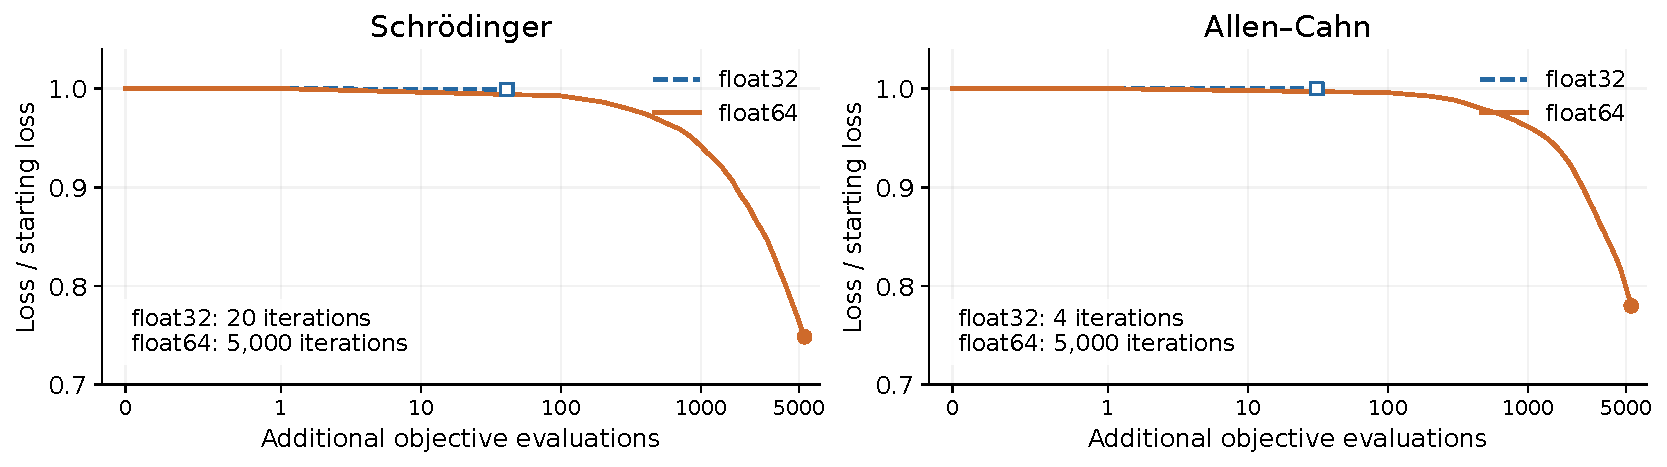
\includegraphics[width=\linewidth]{images/precision_loss.pdf}
\caption{Continuation loss divided by its starting value. Lines connect logged evaluations; markers show the final models. The horizontal axis is logarithmic above one evaluation.}\label{fig:loss}
\end{figure}
Relative to float32 continuation, float64 reduced the Schr\"odinger amplitude error by 5.0\%, its complex error by 7.8\%, and the Allen--Cahn error by 19.0\% (Table~\ref{tab:errors}). Float32 stopped on the relative objective-decrease criterion after 20 and four iterations. Both float64 runs reached 5,000 iterations with lower losses, before reaching the gradient tolerance.

Total runtime mainly reflected how many evaluations were completed. Schr\"odinger used 41 evaluations in float32 and 5,492 in float64; Allen--Cahn used 31 and 5,456. From the logged elapsed times, excluding startup, the average cost per loss-and-gradient evaluation was about 0.26 s in both precisions for Schr\"odinger (RTX 3090), and 0.052 s versus 0.065 s for Allen--Cahn (RTX 2080 Ti). Each pair used the same GPU. The longer float64 runs therefore do not measure the cost of precision alone.

\section{Conclusion and reproducibility}
The PyTorch implementation reproduced the two forward examples at the paper's reference accuracy. Switching to float64 during refinement reduced the errors further, with a larger relative gain for Allen--Cahn. For these runs, precision affected how far L-BFGS-B could progress after the float32 baseline stopped.

The repository includes the code, datasets, configurations, trained weights, and loss histories. \par\textbf{Code and data:} \projectlink

\begingroup\small
\renewcommand{\refname}{References}
\begin{thebibliography}{9}\setlength{\itemsep}{1pt}\setlength{\parskip}{0pt}
\bibitem{raissi} M. Raissi, P. Perdikaris, and G. E. Karniadakis. Physics-informed neural networks: A deep learning framework for solving forward and inverse problems involving nonlinear partial differential equations. \emph{J. Comput. Phys.}, 378:686--707, 2019. \href{https://doi.org/10.1016/j.jcp.2018.10.045}{doi:10.1016/j.jcp.2018.10.045}.
\bibitem{code} M. Raissi. \emph{PINNs: official code and datasets}. \url{https://github.com/maziarraissi/PINNs}, commit \texttt{932f50a2d8ef}.
\end{thebibliography}
\endgroup
\end{document}
